
\documentclass[11pt]{article}

% for footnotes
\makeatletter
\newcommand\footnoteref[1]{\protected@xdef\@thefnmark{\ref{#1}}\@footnotemark}
\makeatother

\usepackage{common}
\usepackage{macros}
\usepackage{nameref}
\usepackage{pdflscape}

\title{HW1: Classification}
\author{Jiafeng Chen\footnote{Equal contribution} \and Yufeng Ling \and
Francisco Rivera$^{*}$}
\begin{document}

\maketitle{}
\section{Introduction}

This note lays out our expectation for a homework submission in
\textit{CS287: Statistical Natural Language Processing}. While you do
not have to follow this template to the letter, we do expect that
write-ups have a very clear structure and cover all the elements
described in this note. With this in mind, the burden is on the
presenter to demonstrate why deviations from the standard are
necessary.

All write-ups should include a short introduction. In this section you
should summarize the underlying problem in high-level language and
describe the extensions that you have decided to propose in your
implementation. When you describe these extensions you should
carefully cite the papers of interest. For instance, it will often be
useful to cite the work seen in class
\citep{murphy2012machine}. Alternatively, you can also cite papers
inline, for instance the work of \citet{berger1996maximum}.


\section{Problem Description---Old}

In general, homeworks will be specified using informal
language. As part of the assignment, we expect you to write-out a
definition of the problem and your model in formal language. For this
class, we will use the following notation:

\begin{itemize}
\item $\boldb, \boldm$;  bold letters for vectors.
\item $\boldB, \boldM$;  bold capital letters for matrices.
\item $\mcB, \mcM$;  script-case for sets.
\item $b_i, x_i$; lower case for scalars or indexing into vectors.
\end{itemize}


For instance in natural language processing, it is common to use
discrete sets like $\mcV$ for the vocabulary of the language, or $\mcT$ for a
tag set of the language.  We might also want one-hot vectors
representing words. These will be of the type
$\boldv \in \{0,1\}^{|\mcV|}$. In a note, it is crucial to define the
types of all variables that are introduced. The problem description is the
right place to do this.

% NLP is also
% full of sequences. For instance sentences, $w_1, \ldots, w_N$, where
% here $N$ is a constant length and $w_i \in \mcV$ for all
% $i \in \{1, \ldots N\}$. If we pretend sentences are all the same
% length, we can have scoring function over sentences,
% $s : \mcV^N \mapsto \reals$.  One might be defined as:

% \[ s(w_1, \ldots, w_N) = \sum_{i = 1}^N p(w_i | w_{i-2}, w_{i-1}), \]

% \noindent where $p$ is the bigram probability, which we will cover later in
% the class.

\section{Problem Description}

The focus of the problem set is sentiment classification. We are given
\emph{sentences} and aim to classify them as either positive or negative
sentiment (a binary classification). These predictions can be made in a
probabilistic fashion by writing $y_i$ as the event that the $i$th sentence is
positive sentiment, and calculating $p(y_i)$.

Sentences\footnote{We use \emph{sentences} to mean a unit of data, which can in
principle be multiple grammatical sentences.} are themselves sequences of words
$w \in \mcV$ in some vocabulary
$\mcV$. In particular, there will be two special words, $w_\text{unk},\,
w_\text{pad} \in \mcV$ which represent an unknown word and a padding unit
respectively; we address their significance later. A particular sequence of
words $w_1, \ldots, w_n$ need not have a fixed length, which varies
across sentences. 

We represent words in two main ways. The first is as a one-hot encoded vector
$\boldv \in \{0,1\}^{|\mcV|}$. This representation is useful for the
\nameref{subsec:logistic} model. Alternatively, we can use a dense embedding.
That is, each word gets assigned a vector $\boldv \in \mathbb{R}^d$ where $d$ is
the embedding dimension. We use \citet{mikolov2013efficient}'s pre-trained word
embeddings ($d=300$) for the \nameref{subsec:cbow} and \nameref{subsec:convnet}
models.


\section{Model and Algorithms}
\label{sec:models}

\subsection{Naive Bayes}
\label{subsec:nb}

\subsection{Logistic Regression}
\label{subsec:logistic}

In this model,  we consider the bag-of-words transform \[x_i = \phi
(w_1^i,\ldots,w_n^i) =
\sum_{j=1}^{n_i} \mathsf{onehot}(w_j),\] and assume that \[
y_i \sim \Bern(p_i) \quad p_i = \sigma(Wx_i),
\]
for the sigmoid function \[
\sigma(t) = \frac{1}{1+e^{-t}}. 
\]
The model is estimated via maximum likelihood over parameter matrix $W$. We
maximize log likelihood via the Adam optimizer in a batched gradient descent
setting, with a learning rate of $10^{-4}$
and weight decay of $10^{-4}$ for 20 epochs. 



\subsection{Continuous Bag of Words}
\label{subsec:cbow}

A downside of logistic regression is that we have as many parameters as the size
of our vocabulary $\mcV$. This means that without an extensive training set, we
run the risk of overfitting. To address this, we can reduce the dimensionality
of our embedding by using \citet{mikolov2013efficient}'s word embeddings. This model has three parts:

\begin{enumerate}
\item We start by using average-pooling over time on the word-embeddings to get
a vector of dimension $d$ for each sentence.
\item Then, we pass that vector through a linear transform to get another vector
of dimension $d_2$ which then gets passed through a non-linear transformation
(ReLU) to make up the hidden layer.
\item Finally, we pass the hidden layer output through another linear layer to
get a vector with two elements, and a softmax transformation to turn these
values into the probabilities of positive and negative sentiment.
\end{enumerate}

The model has two parameter matrices of size $d \times d_2$ and $d_2 \times 2$
respectively. We implement the model for $d_2=100$. We train using Adam for 20
epochs. In summary, the model's steps are visualized in \cref{fig:cbow}.

\begin{figure}[htb]
\centering
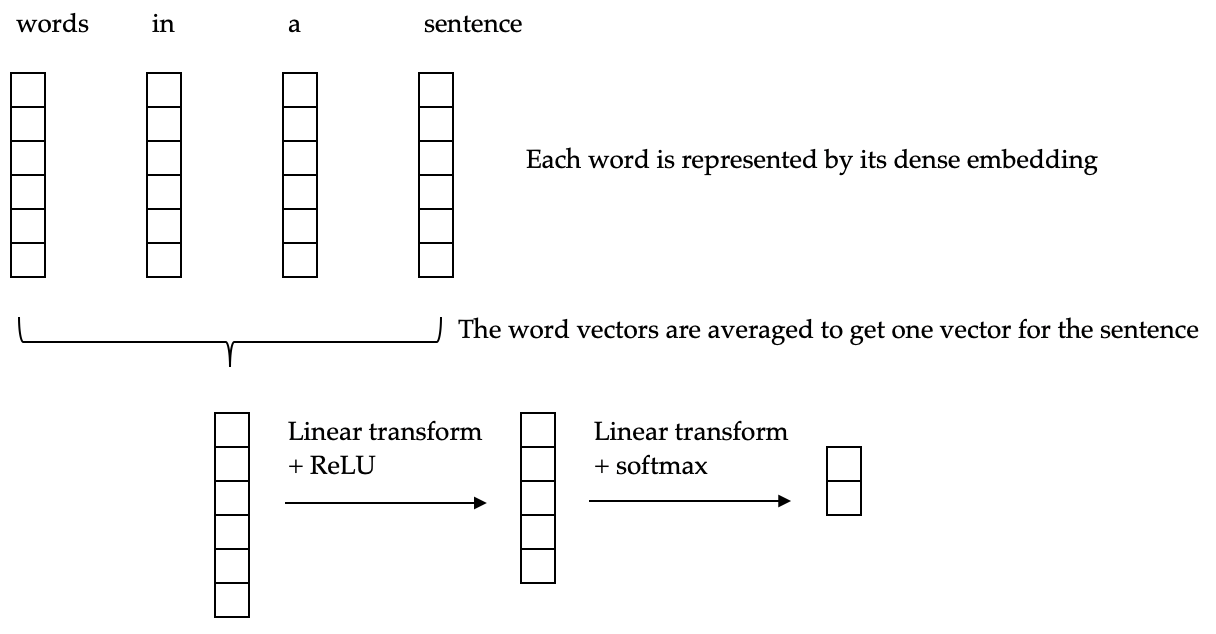
\includegraphics[width=\textwidth]{figs/cbow}
\caption{CBOW model pipeline}
\label{fig:cbow}
\end{figure}

We call this model a \emph{bag of words} because the order of the words is lost
in the average-pooling over time. In other words, any permutation of a sentence
will result in the same prediction by this model. 

\subsection{Convolutional Neural Network}
\label{subsec:convnet}

While the \nameref{subsec:cbow} model makes use of the pre-trained dense
embeddings, it suffers a limitation from the bag-of-words construction. Because
the order of words is not taken into account, the sentences ``it bad, not good''
and ``it good, not bad'' cannot be distinguished. 

\begin{figure}[htb]
\centering
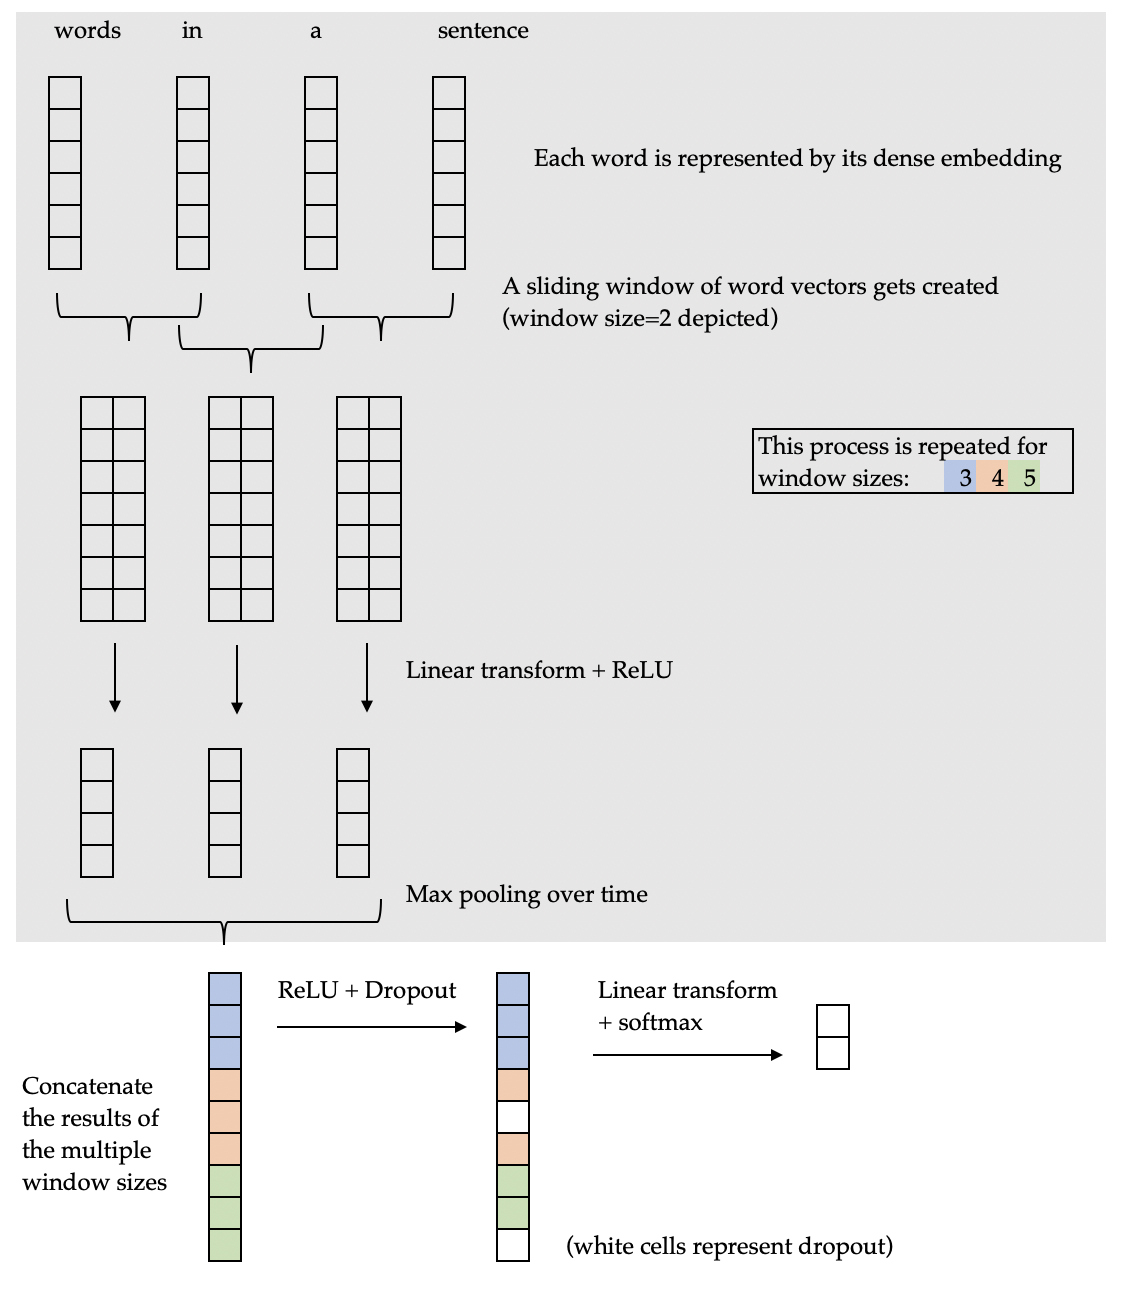
\includegraphics[width=\textwidth]{figs/convnet.png}
\caption{Convolutional Neural Network Model}
\label{fig:convnet}
\end{figure}

% \section{Model and Algorithms---Old}
% 
% Here you specify the model itself. This section should formally
% describe the model used to solve the task proposed in the previous
% section. This section should try to avoid introducing new vocabulary
% or notation, when possible use the notation from the previous section.
% Feel free to use the notation from class, but try to make the note
% understandable as a standalone piece of text.
% 
% This section is also a great place to include other material that
% describes the underlying structure and choices of your model, for
% instance here are some example tables and algorithms from full
% research papers:
% 
% 
% 
% \begin{itemize}
% \item diagrams of your model,
% 
%   \begin{center}
%     \includegraphics[width=0.4\textwidth]{network}
%   \end{center}
% \item feature tables,
% 
%   \begin{center}
%     \begin{tabular}{@{}lll@{}}
%       \toprule
%       &\multicolumn{2}{c}{Mention Features  } \\
%       & Feature & Value Set\\
%       \midrule
%       & Mention Head & $\mcV$ \\
%       & Mention First Word & $\mcV$ \\
%       & Mention Last Word & $\mcV$ \\
%       & Word Preceding Mention & $\mcV$ \\
%       & Word Following Mention & $\mcV$\\
%       & \# Words in Mention & $\{1, 2, \ldots \}$ \\
%       & Mention Type & $\mathcal{T}$ \\
%       \bottomrule
%     \end{tabular}
%   \end{center}
% 
% \item pseudo-code,
% 
%   \begin{algorithmic}[1]
%     \Procedure{Linearize}{$x_1\ldots x_N$, $K$, $g$}
%     \State{$B_0 \gets \langle (\langle \rangle, \{1, \ldots, N\}, 0, \boldh_0, \mathbf{0})  \rangle$}
%     \For{$m = 0, \ldots, M-1$ }
%     \For{$k = 1, \ldots, |B_m|$}
%     \For{$i \in \mcR$}
%     \State{$(y, \mcR, s, \boldh) \gets \mathrm{copy}(B_m^{(k)})$}
%     \For{word $w$ in phrase $x_i$}
%     \State{$y \gets y $ append $w$ }
%     \State{$s \gets s + \log q(w, \boldh) $ }
%     \State{$\boldh \gets \delta(w, \boldh)$}
%     \EndFor{}
%     \State{$B_{m+|w_i|} \gets B_{m+|w_i|} + (y, \mcR - i, s,   \boldh)$}
%     \State{keep top-$K$ of $B_{m+|w_i|}$ by $f(x, y) + g(\mcR)$}
%     \EndFor{}
%     \EndFor{}
%     \EndFor{}
%     \State{\Return{$B_{M}^{(k)}$}}
%     \EndProcedure{}
%   \end{algorithmic}
% 
% \end{itemize}
% 

\section{Experiments}

Finally we end with the experimental section. Each assignment will make clear
the main experiments and baselines that you should run. For these experiments
you should present a main results table. Here we give a sample
Table~\ref{tab:results}. In addition to these results you should describe in
words what the table shows and the relative performance of the models.

Besides the main results we will also ask you to present other results
comparing particular aspects of the models. For instance, for word
embedding experiments, we may ask you to show a chart of the projected
word vectors. This experiment will lead to something like
Figure~\ref{fig:clusters}. This should also be described within the
body of the text itself.

\begin{landscape}
  \begin{table}[t]
\centering
\begin{tabular}{rcccc}
\toprule
{} & Training Accuracy &  Training Average Loss & Validation Accuracy &  Validation Average Loss \\
\midrule
Naive Bayes    &             95.0\% &                 0.0139 &               79.4\% &                   0.0504 \\
Logistic       &             98.8\% &                 0.0131 &               78.2\% &                   0.0487 \\
Embedding NN   &             75.5\% &                 0.0497 &               70.8\% &                   0.0605 \\
CNN            &             98.3\% &                 0.0122 &               76.5\% &                   0.0523 \\
Ensemble       &             98.5\% &                 0.0121 &               80.3\% &                   0.0429 \\
Ensemble-votes &             98.7\% &                    --- &               80.2\% &                      --- \\
\bottomrule
\end{tabular}
\caption{\label{tab:results} Accuracy and average loss (under cross-entropy loss
function) for models considered. Note that for Ensemble, the ensemble weights
are
trained over the validation set and for the model Ensemble-votes, the loss
cannot be computed since model does not output likelihood.}
\end{table}


\end{landscape}

\begin{figure}
  \centering
  \includegraphics[width=6cm]{cluster_viz}
  \caption{\label{fig:clusters} Sample qualitative chart.}
\end{figure}


\section{Conclusion}

End the write-up with a very short recap of the main experiments and the main
results. Describe any challenges you may have faced, and what could have been
improved in the model.

\bibliographystyle{apalike}
\bibliography{writeup}

\end{document}
